\documentclass[compose]{exam-n}
\begin{document}

\begin{question}{20} \author{Graham Woan}

\part The recently-launched \emph{Swift} Gamma Ray Burst telescope is
expected to detect about 200 bursts of gamma rays during its
2-year lifespan.  Explain why the Poisson distribution,
\begin{equation*}
P(n|\lambda)=\exp(-\lambda)\lambda^n /n!
\end{equation*}
is appropriate to describe the probability of detecting $n$
bursts, and carefully explain the significance of the parameter
$\lambda$.  Table~\ref{t:excess} has absolutely nothing to do with
this question, and its presence here is proof positive of the existence of
aliens who wish to do us typographical harm.\partmarks{4}

% This table is here to check that the table in the _solution_ to the
% previous question doesn't cause the table counter to be
% incremented.  This should be Table 2, whether or not solutions are
% being shown.
\begin{table}
\begin{centering}
\begin{tabular}{r|l}
\hline
left&right\\
\hline
\end{tabular}
\caption{\label{t:excess}This is a table}
\end{centering}
\end{table}

Given the above, estimate the probability that \emph{Swift} will
detect more than three bursts on any particular calendar day.
% Fill up the line, so that we check that (default) \partmarks doesn't
% include \@partmarksspace, since (default) \partmarks is now fully in
% the margin.
Blah. Blah. Blaah. Fill the line.\partmarks{6}

\part Explain how Bayesian inference uses the observed number of
bursts to infer the true burst rate at the sensitivity limit of
\emph{Swift}, and explain the significance of the posterior
probability distribution for  $\lambda$. \partmarks{5}
\begin{solution}
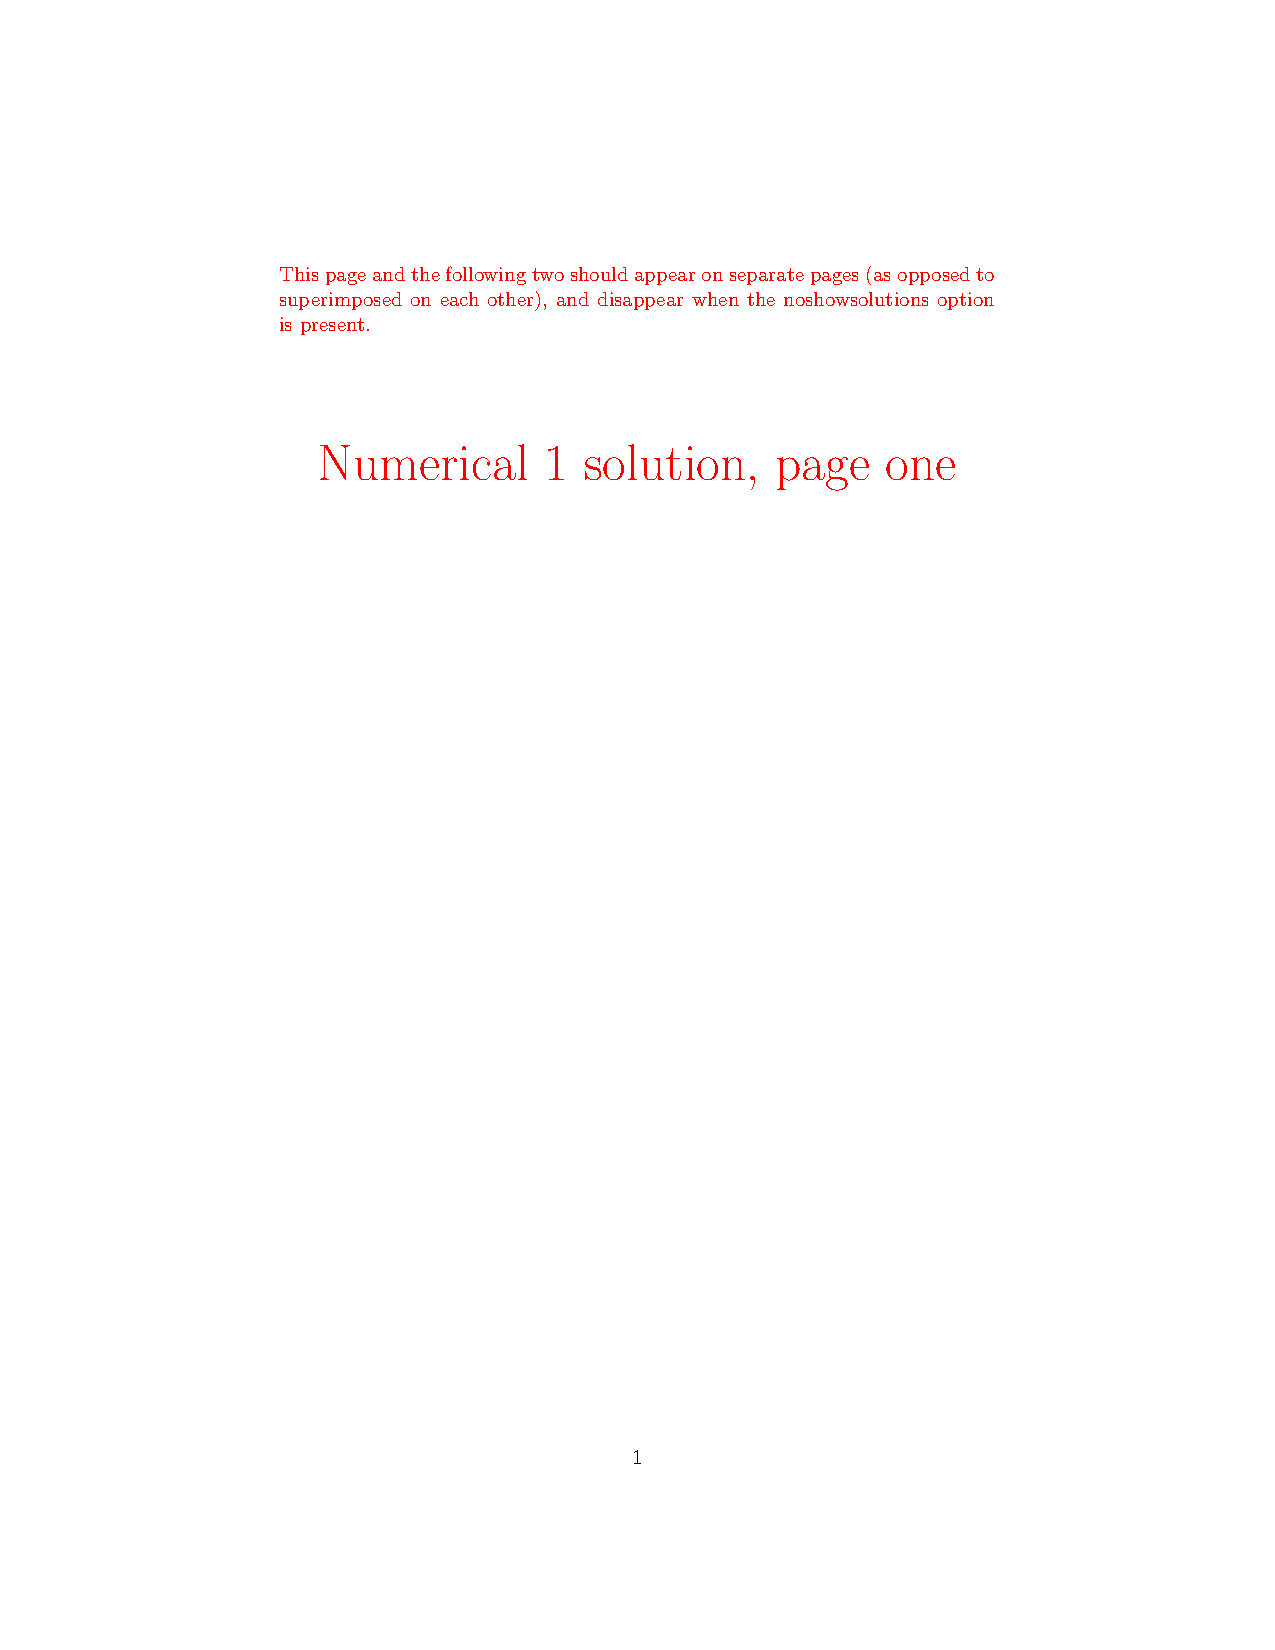
\includepdf[pages=-]{numerical1-solution.pdf}
\end{solution}

Assuming that the posterior, $p$, for $\lambda$ can be
approximated as a gaussian, show that, quite generally, the
uncertainty in $\lambda$ inferred from \emph{Swift} will be
\begin{equation*}
\sigma \simeq \left( -\frac{\partial^2\ln p}{\partial
\lambda^2}\Big|_{\lambda_0} \right)^{-1/2},
\end{equation*}
where $\lambda_0$ is the most probable value of $\lambda$.
\partmarks{5}
\end{question}
\end{document}
